\chapter{Diseño de la interfaz} \label{cap:diseño_interfaz}

 \section{Introducción}

En este capítulo se abordará el diseño de cada uno de los componentes que forman la interfaz de la aplicación SimAS 3.0. Esta versión representa una evolución significativa respecto a las versiones anteriores, incorporando mejoras sustanciales tanto en funcionalidad como en experiencia de usuario.

La interfaz de SimAS 3.0 ha sido completamente rediseñada con un enfoque moderno y profesional, integrando las mejores prácticas de diseño de interfaces gráficas. Se ha implementado un sistema avanzado de pestañas que permite trabajar simultáneamente con múltiples gramáticas y simulaciones, mejorando significativamente la productividad del usuario. El manejo inteligente de ventanas secundarias facilita la comparación de resultados y el trabajo paralelo, características que no estaban disponibles en versiones anteriores.

Uno de los aspectos más destacados es la incorporación de acciones contextuales intuitivas, con iconos descriptivos que representan fielmente las operaciones que realizan. La interfaz presenta un aspecto formal y elegante, con una paleta de colores coherente y una tipografía legible que facilita la lectura prolongada. La navegación se ha optimizado mediante atajos de teclado estratégicos y un sistema de menús jerárquicos que agrupan las funcionalidades de manera lógica.

La aplicación ha sido estructurada siguiendo el patrón Modelo-Vista-Controlador (MVC) \cite{mvc-pattern}, donde el módulo de vistas (implementado en clases como \texttt{MenuPrincipal.fxml}, \texttt{Editor.fxml}, \texttt{PanelSimulacion.fxml}) se encarga de la presentación e interacción con el usuario, proporcionando una separación clara entre la lógica de negocio y la interfaz gráfica.

Se ha prestado especial atención a la accesibilidad y usabilidad, incorporando características como soporte multiidioma completo, indicadores visuales claros para el estado de las operaciones, y validación en tiempo real de las entradas del usuario. La interfaz se adapta automáticamente a diferentes resoluciones de pantalla, manteniendo una experiencia consistente en diversos entornos de trabajo.

Puesto que muchos componentes son similares, se mostrará únicamente un componente de cada tipo en este capítulo técnico. Una descripción más detallada de cada componente de la interfaz, orientada al usuario final, se puede consultar en el \textit{Manual de Usuario}.

A continuación se muestran los elementos gráficos de la interfaz final de la aplicación con una explicación detallada de cada una de las partes que los componen, destacando las innovaciones técnicas implementadas.

\section{Menú principal}

El menú principal constituye la interfaz de entrada principal a la aplicación SimAS 3.0, sirviendo como punto de acceso centralizado a todas las funcionalidades del sistema. Diseñado con una arquitectura modular clara, este componente actúa como un hub de navegación que facilita el acceso intuitivo a los diferentes módulos de la aplicación.

Desde el menú principal, el usuario puede acceder directamente a los módulos principales del sistema: el \textit{Editor de gramáticas}, el \textit{Simulador descendente}, el \textit{Manual de Usuario} y el \textit{Tutorial interactivo}. Esta estructura jerárquica permite una navegación eficiente, reduciendo la curva de aprendizaje y mejorando la experiencia del usuario.

Una de las características más destacadas del menú principal es su diseño responsivo, que se adapta automáticamente a diferentes resoluciones de pantalla manteniendo la legibilidad y funcionalidad. El sistema incorpora indicadores visuales claros que guían al usuario en la selección de opciones, con iconos descriptivos que representan fielmente las operaciones disponibles.

El menú principal implementa un sistema de navegación inteligente que incluye validación de permisos y estados del sistema, asegurando que solo se muestren las opciones disponibles en cada momento. Esta característica es especialmente importante en un entorno educativo donde los usuarios pueden tener diferentes niveles de experiencia.

Además, el menú principal incluye un selector de idioma integrado que permite cambiar dinámicamente el idioma de toda la interfaz, característica que demuestra la internacionalización completa implementada en SimAS 3.0. Los textos se actualizan en tiempo real sin necesidad de reiniciar la aplicación.

En la figura \ref{fig:d1}, se muestra el menú principal de SimAS con sus elementos principales: el título de la aplicación, los botones de navegación principales, el selector de idioma y la información del desarrollador.

\needspace{8cm}
\begin{figure}[H]
\centering
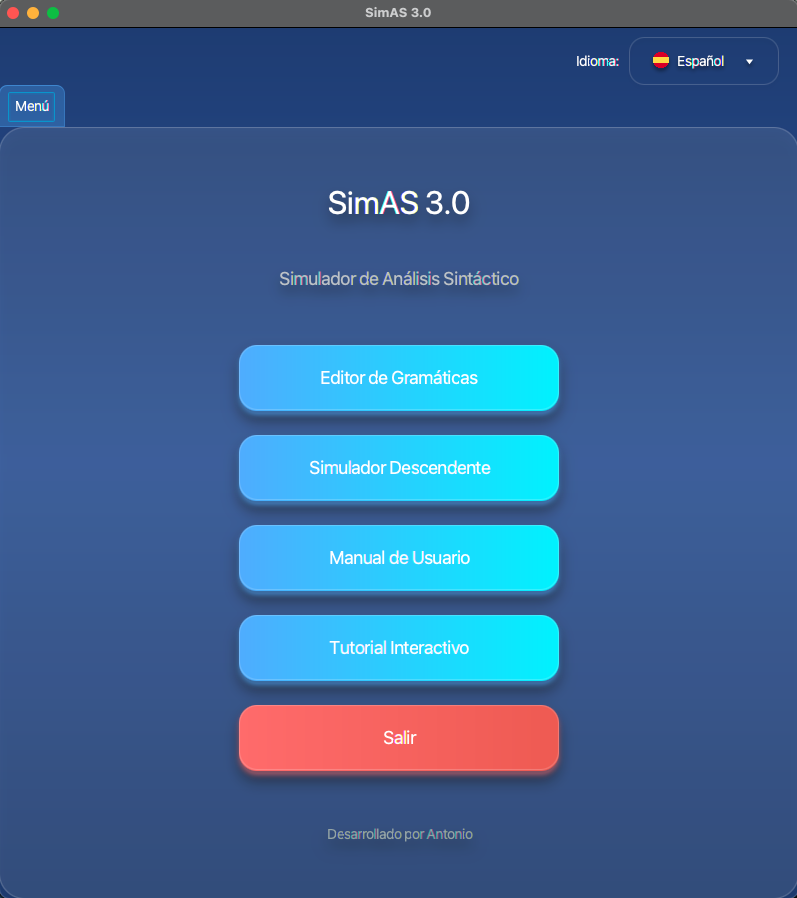
\includegraphics[width=0.8\textwidth]{figuras2/menu.png}
\caption{Menú principal de SimAS.}
\label{fig:d1}
\end{figure}

El menú principal mantiene una estructura consistente y predecible que facilita la navegación, agrupando las funcionalidades relacionadas de manera lógica. Esta organización refleja la arquitectura modular del software, donde cada módulo mantiene su independencia mientras colabora eficientemente con los demás componentes del sistema. 

\section{Barras de herramientas}

Las barras de herramientas constituyen uno de los elementos más importantes de la interfaz de usuario en SimAS 3.0, proporcionando acceso directo e intuitivo a las funciones más utilizadas del sistema. Implementadas como componentes gráficos interactivos, estas barras mejoran significativamente la eficiencia del usuario al reducir la necesidad de navegar por menús complejos.

En el contexto del Editor de gramáticas, la barra de herramientas juega un papel fundamental al ofrecer accesos directos a todas las operaciones relacionadas con la creación, edición y gestión de gramáticas. Esta implementación sigue los principios de diseño de interfaces modernas, priorizando la usabilidad y la accesibilidad.

Una característica técnica destacada de la barra de herramientas es su comportamiento dinámico de habilitación/deshabilitación de controles. Al abrir inicialmente el editor, solo un conjunto limitado de botones permanece activo, específicamente los botones \textbf{Nueva}, \textbf{Abrir} y \textbf{Salir}. Esta estrategia de diseño inteligente previene errores del usuario y guía el flujo de trabajo de manera natural.

En la figura \ref{fig:d2a}, se muestra el estado inicial de la barra de herramientas, donde la mayoría de los controles aparecen deshabilitados para evitar operaciones prematuras.

\needspace{3cm}
\begin{figure}[H]
\centering

\includegraphics[width=0.8\textwidth]{figuras2/editor/barra_herramientas_deshabilita_parcial.png}
\caption{Barra de herramientas con controles parcialmente deshabilitados (estado inicial).}
\label{fig:d2a}
\end{figure}

Una vez que se carga o crea una gramática en el editor, el sistema habilita automáticamente el resto de los controles, permitiendo al usuario acceder a todas las funcionalidades disponibles. Esta transición inteligente refleja la arquitectura de estados del sistema, donde la interfaz se adapta dinámicamente según el contexto de uso.

En la figura \ref{fig:d2}, se muestra la barra de herramientas completamente funcional una vez que se ha cargado una gramática.

\needspace{3cm}
\begin{figure}[H]
\centering

\includegraphics[width=0.8\textwidth]{figuras2/editor/barra_herramientas.png}
\caption{Barra de herramientas completamente funcional.}
\label{fig:d2}
\end{figure}

El diseño de los iconos sigue una convención sistemática que facilita el aprendizaje y la memorización. Se ha procurado que cada botón sea descriptivo y represente fielmente la operación que realiza. Para lograr esto, se ha implementado un sistema de iconos compuesto por una forma base que identifica el objeto involucrado en la operación, complementada con una forma secundaria que representa la acción específica.

Por ejemplo, las operaciones relacionadas con gramáticas están representadas con la letra \textit{G} como forma base, mientras que las operaciones de simulación utilizan la letra \textit{S}. A esta forma base se le superpone gráficamente la acción a realizar, siempre posicionada en la esquina superior derecha del icono. Esta composición visual permite una identificación rápida y precisa de las funcionalidades disponibles.

Esta estrategia de diseño no solo mejora la intuitividad de la interfaz, sino que también optimiza el espacio disponible y reduce la carga cognitiva del usuario. El sistema de habilitación contextual asegura que los usuarios se centren en las tareas apropiadas para cada etapa del proceso, mejorando tanto la eficiencia como la calidad del trabajo realizado.
  

\section{Ventana del editor}

La ventana del editor representa el módulo principal de creación y gestión de gramáticas en SimAS 3.0. Este componente se abre en una nueva pestaña independiente cuando el usuario selecciona las opciones de crear una nueva gramática o editar una existente desde el menú principal.

El editor proporciona una interfaz completa para el diseño, modificación y validación de gramáticas de contexto libre, facilitando el proceso de preparación de datos para las simulaciones posteriores. Las imágenes mostradas en esta sección corresponden al estado del editor con una gramática activa cargada. Para observar las diferencias con la ventana del editor vacía, se puede consultar el Manual de Usuario.

La ventana del editor está compuesta por los siguientes elementos principales:
\begin{enumerate}
 \item \textbf{Barra de herramientas}: proporciona accesos directos a todas las operaciones disponibles.
 \item \textbf{Información de la gramática}: componentes que muestran la información de la gramática activa.
\end{enumerate}

En la figura \ref{fig:d3}, se muestra un ejemplo completo de la ventana del editor con una gramática activa.

\needspace{8cm}
\begin{figure}[H]
\centering
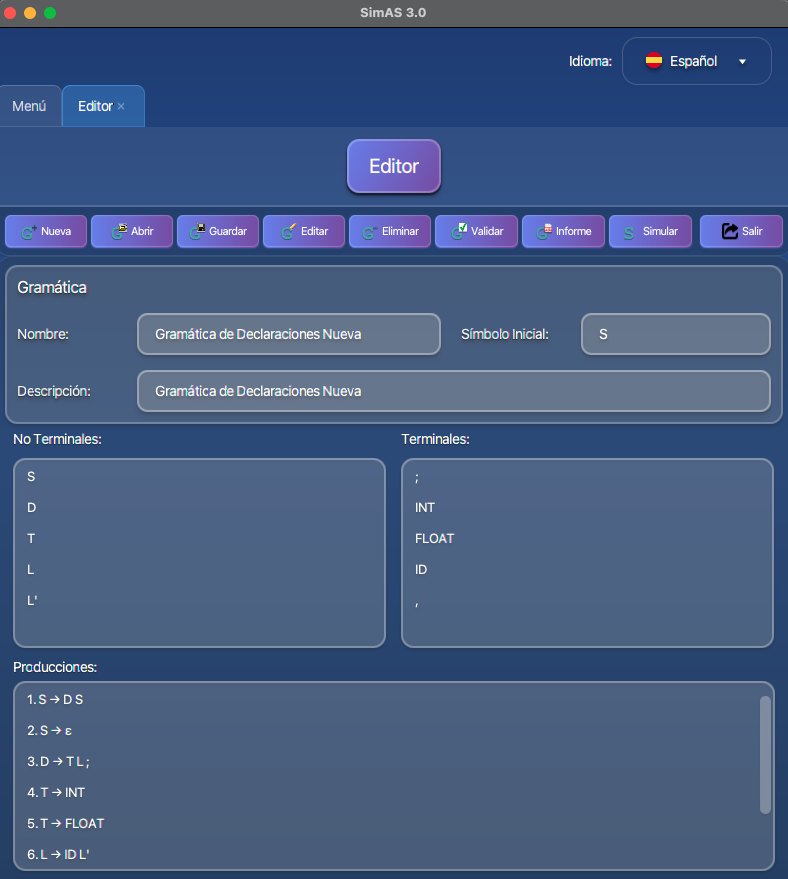
\includegraphics[width=0.9\textwidth]{figuras2/ejemplo_practico/editor.png}
\caption{Ventana del editor con gramática activa.}
\label{fig:d3}
\end{figure}

La barra de herramientas del editor ya fue detallada en la sección anterior, destacando su sistema inteligente de habilitación/deshabilitación de controles. A continuación se describe el panel de edición, que constituye el corazón funcional del módulo de creación de gramáticas.

\subsection{Panel de edición}

El panel de edición constituye el núcleo funcional del módulo de creación de gramáticas, implementando un proceso estructurado de 4 pasos que guía al usuario a través de la definición completa de una gramática de contexto libre. Este proceso asistido asegura que se recopilen todos los elementos necesarios para una gramática válida y funcional.

El proceso de 4 pasos se detalla exhaustivamente en la sección \ref{sec:ventana_asistente} de este mismo capítulo, donde se explica el funcionamiento del asistente de creación de gramáticas. En esta sección se proporciona una visión general de los componentes principales del panel de edición.

Este panel representa la interfaz principal de interacción para la creación y modificación de gramáticas, proporcionando una experiencia de usuario intuitiva y guiada que facilita el proceso de definición de lenguajes formales.

\section{Ventana del simulador}

La ventana del simulador permite ejecutar la simulación de un analizador descendente o ascendente utilizando una gramática. En la figura \ref{fig:d5}, se muestra un ejemplo de esta ventana.

La ventana está compuesta de los siguientes elementos:
\begin{enumerate}
 \item \textbf{Barra de menús}: barra de menús de la ventana.
 \item \textbf{Barra de herramientas}: barra de herramientas de la ventana.
 \item \textbf{Panel de simulación}: panel que muestra los datos de la gramática a simular.
\end{enumerate}

\begin{figure}[htp]
\centering
	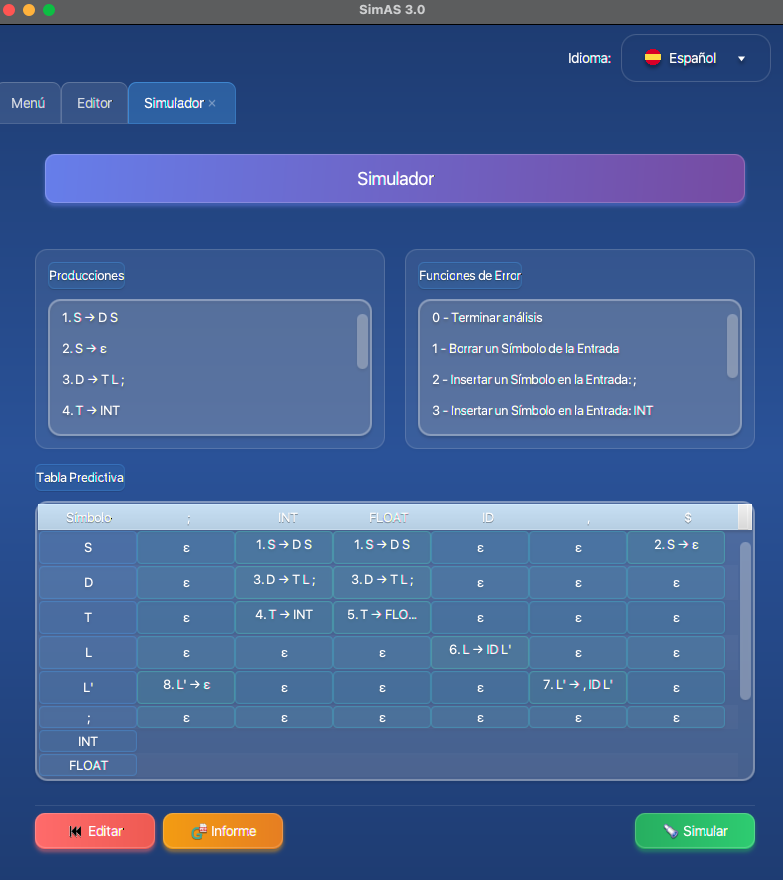
\includegraphics[width=0.8\textwidth]{figuras2/ejemplo_practico/simulador.png}
	\caption{Ventana de simulación.}
	\label{fig:d5}
\end{figure}

  En las secciones anteriores ya se vio con detalle la barra de menús y la barra de herramientas; a continuación, se llevará a cabo la descripción de cada una de las partes que compone el panel de simulación.



\subsection{Panel de simulación}

El panel de simulación permite visualizar las simulaciones de los analizadores sintácticos. En la figura \ref{fig:d6}, se muestra un ejemplo de este panel.

El panel está compuesto de los siguientes elementos:
\begin{enumerate}
 \item \textbf{Tipo de análisis}: muestra el tipo de simulación que se va a llevar a cabo, \textit{descendente} o \textit{ascendente}. En el caso de ser la simulación del análisis ascendente, también se detalla el tipo: \textit{SLR}, \textit{LR-canónico} o \textit{LALR}.
 \item \textbf{Producciones de la gramática}: visualización gráfica de las producciones de la gramática.
 \item \textbf{Funciones de error}: lista de funciones de error de la gramática.
 \item \textbf{Tabla predictiva o tabla LR}: muestra la tabla predictiva o la tabla LR, dependiendo del método seleccionado.
\end{enumerate}

\begin{figure}[htp]
\centering
	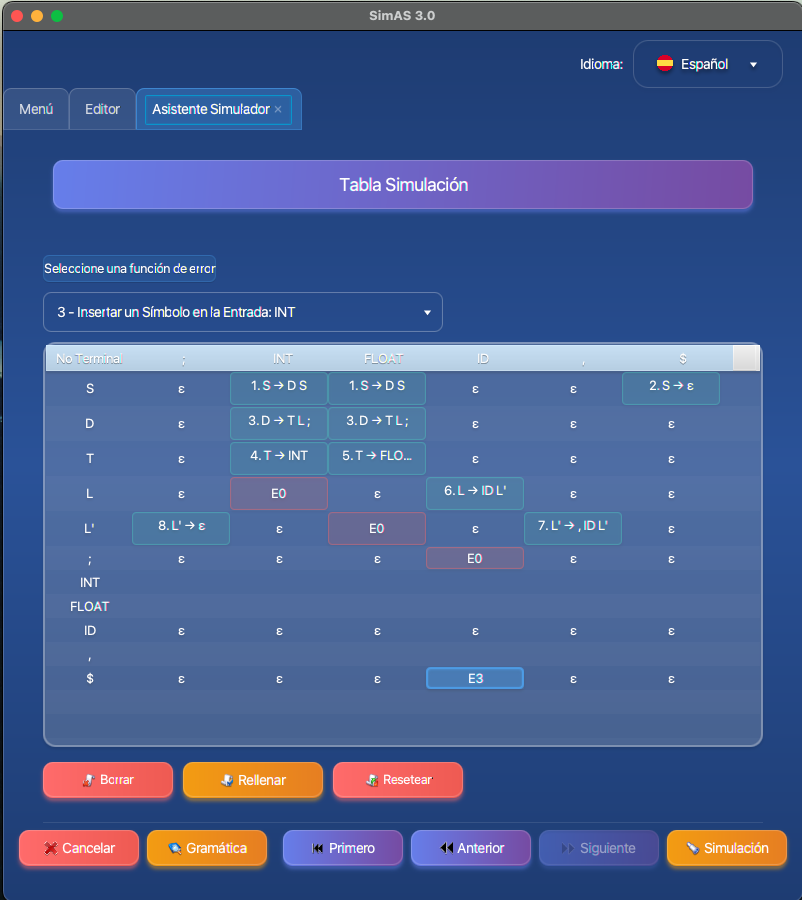
\includegraphics[width=0.8\textwidth]{figuras2/simulador/paso5_tablaPredictivaCompleta.png}
	\caption{Panel de simulación.}
	\label{fig:d6}
\end{figure}

\subsection{Ventana de Gramática Original}

\textbf{Visualización de la Gramática Original} (Novedad): a medida que se generan los diferentes conjuntos, tablas y funciones de error, se le permite al usuario visualizar la gramática original para así poder realizar las comparaciones que desee si dicha gramática se ha transformado en otra porque se ha eliminado la recursividad por la izquierda o se ha factorizado por la izquierda. La ventana será un panel simple donde se muestre la gramática original de la misma forma que se muestra la gramática modificada (Figura \ref{fig:d10}).

\begin{figure}[htp]
\centering
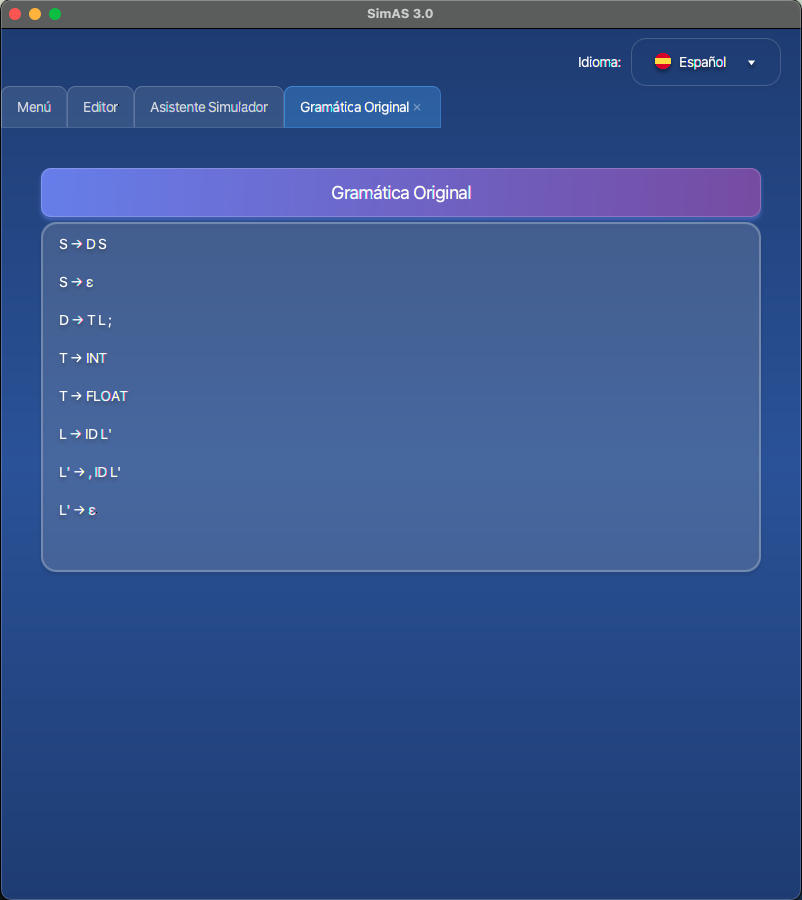
\includegraphics[width=0.8\textwidth]{figuras2/simulador/gramatica_original.png}
\caption{Gramática Original.}
\label{fig:d10}
\end{figure}

 \section{Ventana de simulación}

La ventana de simulación se encarga de ejecutar las simulaciones de una cadena de entrada. En la figura \ref{fig:d7}, se muestra un ejemplo de esta ventana.

La ventana está compuesta de los siguientes elementos:
\begin{enumerate}
  \item \textbf{Tipo de análisis}: muestra el tipo de simulación que se va a llevar a cabo, \textit{descendente} o \textit{ascendente}. En el caso de ser la simulación del análisis ascendente, también se detalla el tipo: \textit{SLR}, \textit{LR-canónico} o \textit{LALR}.
 \item \textbf{Cadena de entrada}: permite introducir los símbolos terminales que forman parte de la cadena de entrada que se va a simular.
 \item \textbf{Botones de Avance y Retroceso}: la simulación se podrá realizar paso a paso o de forma completa, pudiendo avanzar y retroceder en cada paso.
 \item \textbf{Tabla de análisis}: representa la tabla de resultados del análisis.
 \item \textbf{Generar Árbol Sintáctico} (Novedad): permite abrir una ventana en la que se genere el árbol sintáctico correspondiente.
 \item \textbf{Generar Derivación} (Novedad): permite abrir una ventana en la que se genere la derivación de la simulación correspondiente.
 \item \textbf{Informe de la Simulación}: permite al usuario generar un informe en pdf de la simulación.
\end{enumerate}

\begin{figure}[htp]
\centering
	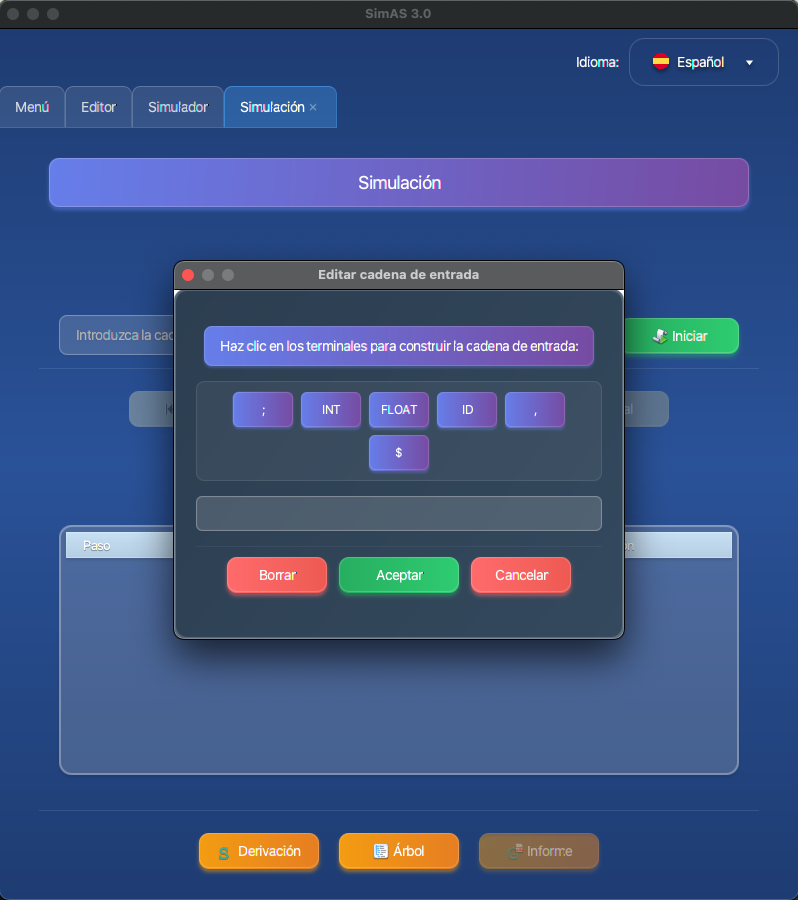
\includegraphics[width=0.8\textwidth]{figuras2/simulador/simulacion_cadenaEntrada.png}
	\caption{Ventana de simulación.}
	\label{fig:d7}
\end{figure}

\section{Ventana de Visualización del Árbol Sintáctico}

El árbol sintáctico se podrá ver en una ventana la cual se irá repintando a medida que se continue con la simulación (Figura \ref{fig:da22}).

\begin{figure}[htp]
\centering
	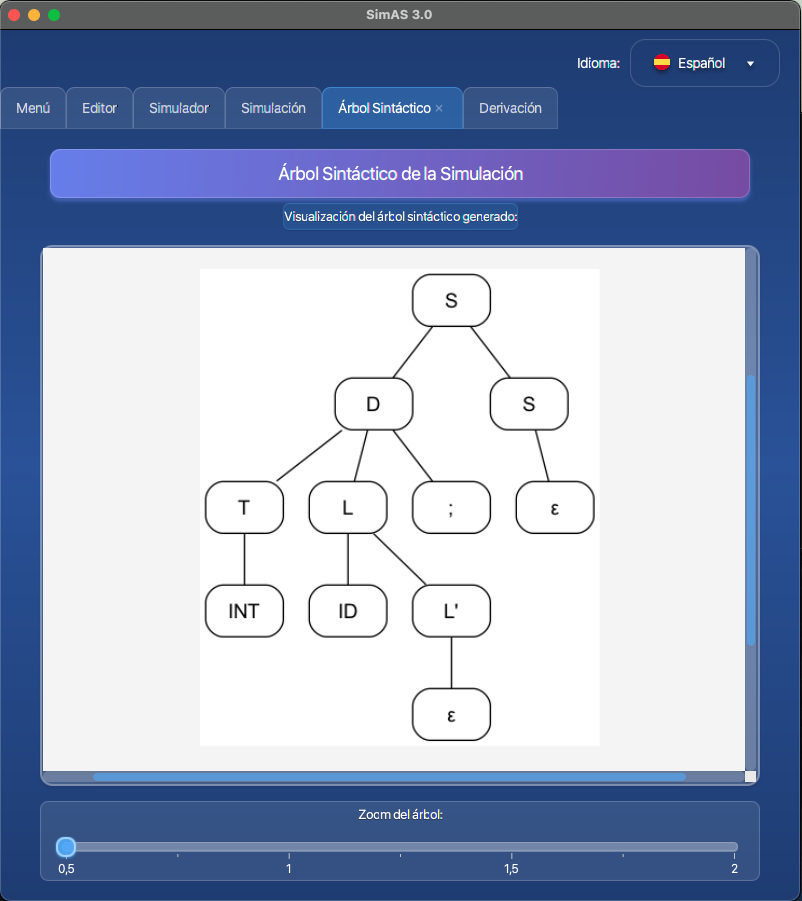
\includegraphics[width=0.8\textwidth]{figuras2/simulador/simulacion_arbol.png}
	\caption{Ventana de simulación.}
	\label{fig:da22}
\end{figure}

 \section{Ventana de Derivación Sintáctica}

Además del árbol, es posible generar la derivación de la simulación actual en una ventana adicional tal y como se muestra en la imagen \ref{fig:da24}:

\begin{figure}[htp]
\centering
	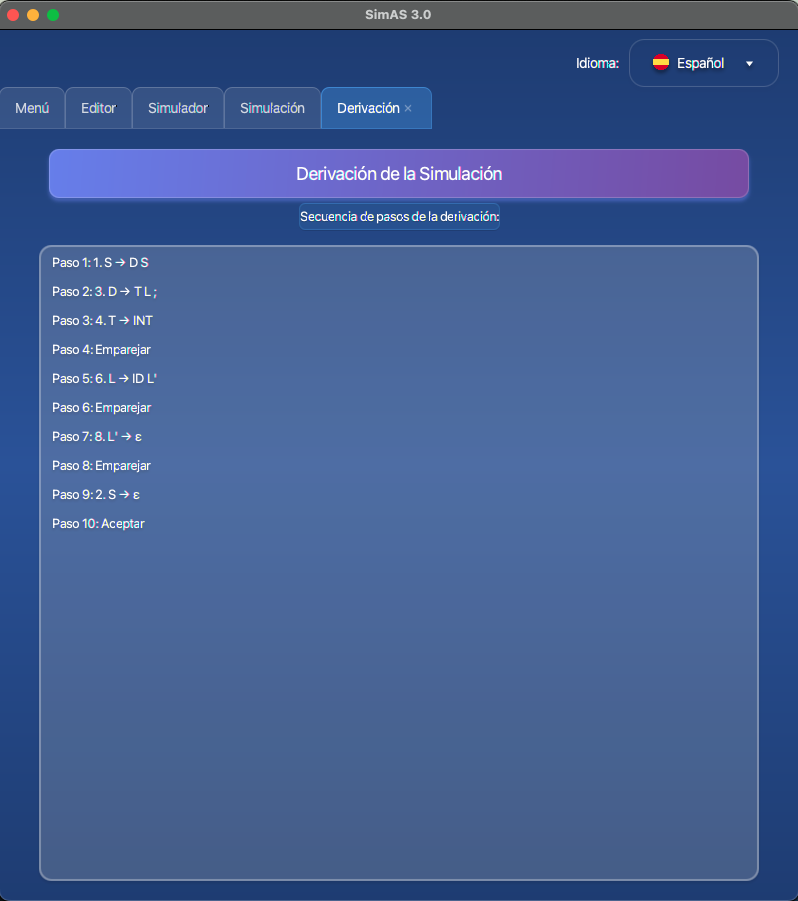
\includegraphics[width=0.8\textwidth]{figuras2/simulador/simulacion_derivacion.png}
	\caption{Ventana de simulación.}
	\label{fig:da24}
\end{figure}

\section{Ventana de asistente} \label{sec:ventana_asistente}

En SimAS se han creado dos tipos de asistentes: el \textit{asistente de creación de una gramática} y el \textit{asistente de creación de una simulación}. En la figura \ref{fig:d8}, se muestra un ejemplo de esta ventana; en concreto, el primer paso del asistente de creación de una gramática.

La ventana está compuesta de los siguientes elementos:
\begin{enumerate}
 \item \textbf{Título}: contiene un título descriptivo de la ventana en la que se sitúe el asistente.
 \item \textbf{Contenido}: información que se muestra en el panel en función del paso en el que se está.
 \item \textbf{Botonera}: permite controlar la evolución del asistente (cancelar, ir al paso anterior, ir al primer paso, etcétera).
\end{enumerate}

\begin{figure}[htp]
\centering
	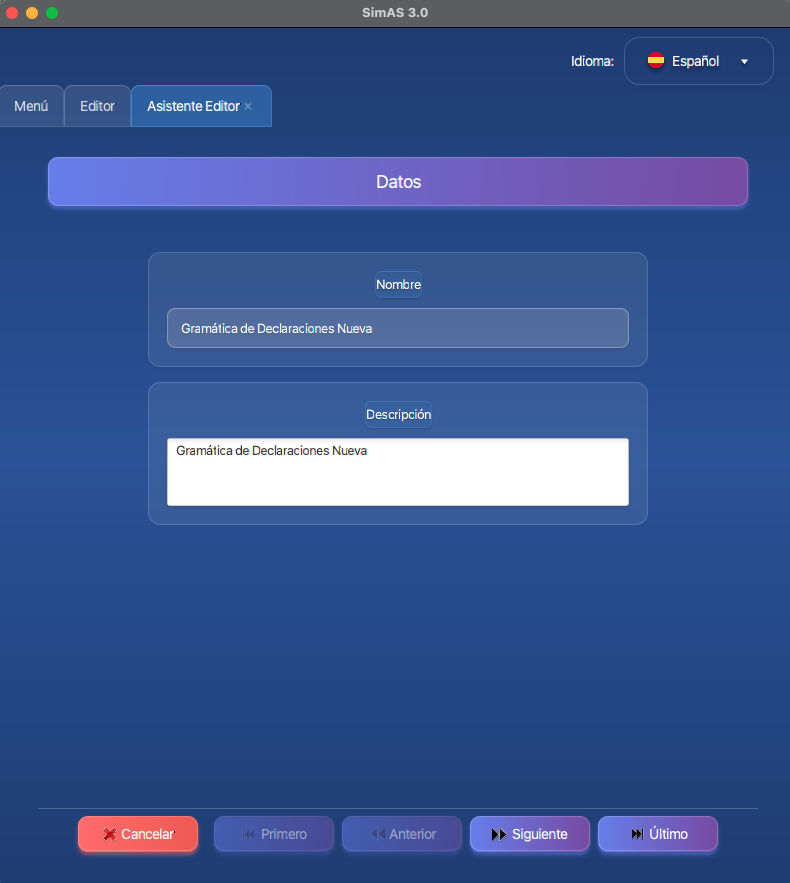
\includegraphics[width=0.8\textwidth]{figuras2/ejemplo_practico/editor_paso1.png}
	\caption{Ventana de asistente.}
	\label{fig:d8}
\end{figure}

\section{Ventanas de edición} \label{sec:ventanas_edicion}

Las ventanas de edición representa a todas las ventanas que permiten realizar una edición de un objeto (nombre, descripción, símbolos, producciones, funciones de error, etcétera). En la figura \ref{fig:d9}, se muestra un ejemplo de esta ventana; en concreto, la ventana de edición de los símbolos de la gramática.

La ventana está compuesta de los siguientes elementos:
\begin{enumerate}
 \item \textbf{Título}: contiene un título descriptivo de la ventana.
 \item \textbf{Contenido}: información a editar que se muestra en la ventana.
 \item \textbf{Botonera}: permite cancelar o aceptar la operación. El botón de cancelar siempre estará situado a la izquierda, mientras que el de aceptar lo estará en la derecha.
\end{enumerate}

\begin{figure}[htp]
\centering
	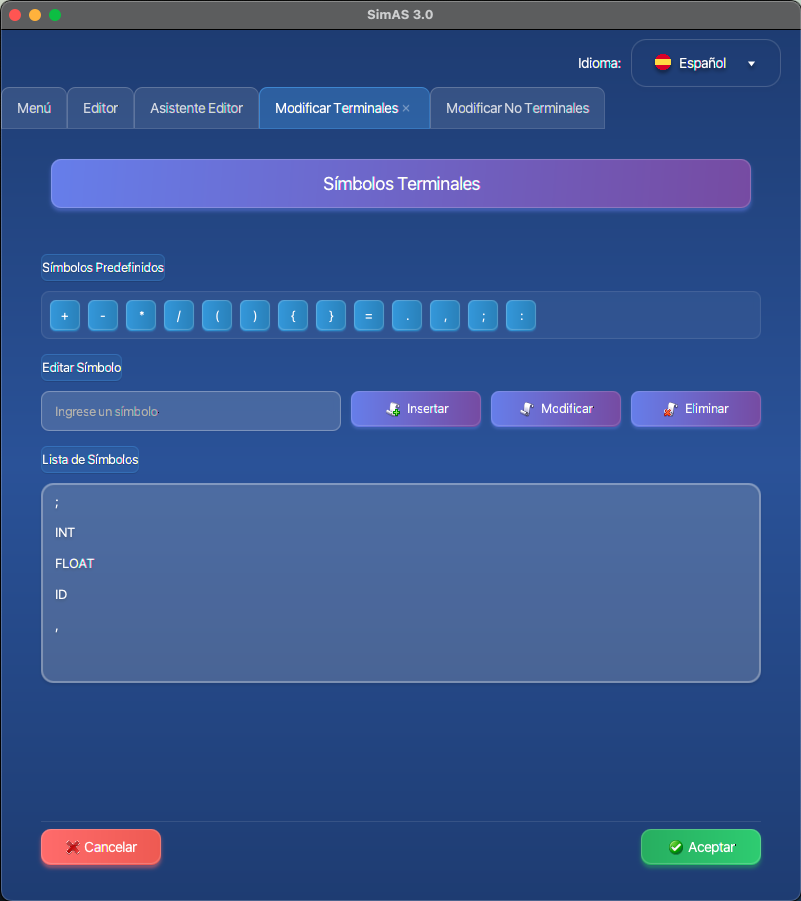
\includegraphics[width=0.8\textwidth]{figuras2/editor/panel_terminales.png}
	\caption{Ventana de edición.}
	\label{fig:d9}
\end{figure}